\chapter{Implementation}
\label{chap:implementation}

The following chapter describes the implementation of the system. Jayes, the third party implementation used for the Bayesian network is briefly presented. We give a detailed description of the \emph{context engine}, which provides developers with a flexible way of supporting new context in the system. The implementation used for communicating with OpenHAB is briefly described and lastly the prototype is presented.

\section{Status}
\label{sec:implementation:status}

As part of the project we have designed and implemented a context-aware home automation solution on an Android Wear and a Raspberry Pi with Philips Hue light bulbs and a desktop machine running a Spotify client acting as the controllable devices. 

\todo[author=Simon]{Evt. indsæt billede af alle de involverede enheder.}

\subsection{Implemented Features}

Below we present the features implemented as part of the project. Features are grouped by the hardware the software is running on.

\subsubsection{Android Wear}

The user utilizes the Android Wear smart watch to perform gestures which starts the context recognition process. Furthermore the smart watch is used for positioning the user and configuring parts of the system. The following features were implemented on the watch.

\begin{itemize}
\item Retrieval of available devices and actions from openHAB.
\item Configuration of the smart watch application based on rooms and beacons registered in openHAB.
\item Training of gestures using the 1\textcent~gesture recognizer as described in \cref{sec:design:gesture-recognition}.
\item Recognition of gestures using the 1\textcent~gesture recognizer.
\item Positioning of the user using Estimotes BLE beacons as described in \cref{sec:design:ble-positioning}.
\item Setup of gesture configurations, i.e. a combination of a gesture, a room and an action.
\item Recognition of the context using a Bayesian network as described in \cref{sec:design:bayesian-network}.
\item Presentation of a list of actions if one single action cannot be determined but rather we have a set of actions to choose from.
\item Configuration and use of virtual positions, i.e. allowing the user to manually determine which room he is in.
\end{itemize}

\subsubsection{Raspberry Pi}

The Raspberry Pi runs openHAB, which was described in \cref{sec:analysis:choice-of-hub}. openHAB is the home automation software utilized in the project. The software receives HTTP requests which is then translated to an equivalent request using an appropriate protocol, e.g. Bluetooth, HTTP or MQTT, and forwards the translated request to a controllable device. The following features were implemented on openHAB.

\begin{itemize}
\item We implemented an openHAB plugin for configuring the relationship beacons and rooms and the relationship between the two.
\item openHAB was configured to support the actions in the scenario presented in \cref{sec:analysis:scenarios}, e.g. we implemented rules to toggle a lamp between the on and off states as this is not directly supported by openHAB.
\end{itemize}

\subsubsection{Desktop Machine}

The desktop machine serve as the media centre used for testing while developing the solution. In order to control Spotify, we developed a smart application that runs on the desktop machine. The application receives requests over HTTP and forwards them to the Spotify client for OS X which is an AppleScript scriptable application, meaning that it provides a terminology that scripts can use to send \emph{events} to the application. An event triggers a handler within the application which in some way modifies the application. For the Spotify application, events includes ``next'', ``previous'' and ``playpause''. When the application receives an event, an appropriate action is taken in the application.

The following feature was implemented in the application running on the desktop machine.

\begin{itemize}
\item Skip to next track, skip to previous track, play and pause the music in Spotify by issuing HTTP requests to the application.
\end{itemize}

\subsection{Missing Implementation}

While not part of the requirements presented in \cref{sec:requirements-specification}, we presented a model for including the state of the system in \cref{sec:design:bayesian-network}. The system state was introduced in the model to illustrate how contextual information different than the gesture performed by the user and the users location can be included in the system.

The following feature was not implemented.

\begin{itemize}
\item Inclusion of the ofsystem state in the Bayesian network used for recognizing the context.
\end{itemize}

While the feature is not implemented, a naive implementation of the system state is trivial to implement. The Android Wear application can periodically request the state of all controllable devices registered in openHAB and based on the response, populate the system state nodes in the Bayesian network with the appropriate states. The nodes will typically have hard evidence on one of the states as openHAB is considered to hold the truth of the systems state, e.g. it knows if a television is on or not and if music is playing or not.

%%% Local Variables:
%%% mode: latex
%%% TeX-master: "../../master"
%%% End:

\section{Programming Languages}
\label{sec:implementation:programming-language}

In order to give a better understanding of the implementation details, we present the programming languages used for the implementation with the reasoning of the language choices.

\subsection{Android Wear}

The primary application presented in this report is an Android Wear application. While Googles Android framework APIs are targeted towards a Java environment, Google do provide Android NDK, a toolset for writing parts of an Android application in the C or C++ programming languages. Google emphasize that Android NDK is intended only for parts of an application and is generally not suited for most applications. The Android SDK is meant to be used when reusing existing code libraries or frameworks written in C or C++.

Alternative tools for developing to the Android platform includes Xamarin\footnote{For more information on Xamarin, refer to \url{https://www.xamarin.com}.} and Phonegap\footnote{For more information on Phonegap, refer to \url{http://phonegap.com}.} in which developers write applications in either C\# or HTML and CSS respectively. The tools are targeted towards cross-platform development, \ie~developing for multiple platforms using the same codebase.

For the purpose of the prototype, we have no interest in supporting other platforms than the Motorola 360. Furthermore we are comfortable with the Java programming language. Therefore we chose write the application in Java.

\subsection{Raspberry Pi}

We developed an addon for the openHAB which runs on the Raspberry Pi. Because openHAB provides a Java based framework for writing addons and we were already writing Java for the Android Wear platform, we decided to write the addon in Java.

\subsection{Desktop Machine}

The small application created for controlling a Spotify clent running on a desktop machine using HTTP requests, was developed in JavaScript using the Node.js framework\footnote{For more information on Node.js, refer to \url{https://nodejs.org}.}. The client calls a script written in AppleScript.

Because the application does not depend on APIs from other services but merely invokes a local AppleScript, the choice of language and framework was based on our familarity with the two.

%%% Local Variables:
%%% mode: latex
%%% TeX-master: "../../master"
%%% End:

\section{Version Control}
\label{sec:implementation:version-control}

We use version control management for keeping track of changes to the codebase developed through the project as well as this report. Below is a list of advantages of using version control management.

\begin{itemize}
\item Collaborators can work on the same file at the same time, due to the way changes to the file can be \emph{merged}. This is in contrary to a shared folder, \eg~a Dropbox folder which always synchronize the most recent version of a file with a central location.
\item Keeping track of what files were changed, what was changed in the files and who changed it.
\item When publishing changes to the files, authors typically tag the changes with a message with a description of the changes making their intention clear to collaborators.
\item Changes can be rolled back to a previous state.
\item Collaborators of a project can \emph{branch} out from the main codebase to create changes without touching the currently stable code base. When their changes are done, they can \emph{merge} in their changes to the stable codebase.
\item Depending on the amount of collaborators and the system used, the codebase is inherently backed up.
\end{itemize}

There are several software solutions for version control management, including Git, Subversion, CVS and Bazaar. When choosing a system to use, we decided to only look into the Git and Subversion as we have experience with the two.

The key difference between Git and Subversion is, that Git is decentralized and Subversion is centralized. When using Git, collaborators have a local copy of the entire repository in which the codebase resides. Collaborators then push their changes to a central location when they are done working on a feature or a fix. With Subversion, collaborators are working in a central online repository, meaning that the version control features are unavailable when there is no connection to the repository.

We chose Git over Subversion because of it being decentralized. This provides two advantages over Subversion.

\begin{itemize}
\item When we are working with no or an unstable internet connection, version control features are still available. Several times during the project we have worked with no internet connection.
\item We believe that a decentralized and local system provides extra safety in terms of backups. All collaborators always have a backup of the repository on their local machines. In addition, we push the changes to GitHub, a website for hosting Git repositories, from which we also pull the changes other collaborators make.
\end{itemize}

%%% Local Variables:
%%% mode: latex
%%% TeX-master: "../../master"
%%% End:

\section{Bayesian Network}
\label{sec:implementation:bayesian-network}

In \cref{sec:analysis:recommender-systems,sec:design:bayesian-network} we described our motivation to use a Bayesian network for determining the appropriate action to trigger given a context. In order to save time on the implementation of the Bayesian network, we decided investigate third party implementations.

Our requirements for the implementation were the following:

\begin{itemize}
\item The implementation should be correct, i.e. given a set of nodes with states, edges, probabilities and evidence the computed belief of the nodes should be correct.
\item The implementation should support soft evidence as described in \cref{sec:design:bayesian-network}.
\item The implementation should be written in Java.
\end{itemize}

We chose to only consider implementations written in Java as we are familiar with the language and we were confident that implementations written in Java would run on Android platforms with only little work required. 

The correctness of the implementation was validated using Hugin, a decision making tool previously described in \todo[author=Simon]{Indsæt reference til beskrivelse af Hugin.}. Given a set of nodes with states, edges, probabilities and evidence on the states, the resulting belief of the states should equal the resulting belief when the same configurations were made in Hugin.

When investigating third party solutions, we found that only few implementations supported soft evidence. Since we utilize this in the design of the Bayesian network, the implementation must support it. 

We found that the Jayes\footnote{The Jayes implementation is available at \url{http://www.eclipse.org/recommenders/jayes/}.} and Bruse\footnote{The Bruse implementation is available at \url{https://github.com/slangevi/bruse}.} implementations fulfilled our requirements. We chose to use the Jayes framework for the following reasons.

\begin{itemize}
\item The framework is maintained by Eclipse Foundation, who use it in Code Recommenders, a tool for intelligent code completion\footnote{More inforrmation aobut the Eclipse Code Recommenders is available at \url{http://www.eclipse.org/recommenders/}.}. The implementation being used in a large project and maintained by a foundation may be the reason it is more widespread and more information, such as documentation, is available.
\item The framework  has unit tests which eases the process of getting started using the framework as the unit tests help document how the framework is intended to be used.
\end{itemize}

%%% Local Variables:
%%% mode: latex
%%% TeX-master: "../../master"
%%% End:

\section{Context Engine}
\label{sec:implementation:context-engine}

In \Cref{sec:design:bayesian-network,sec:design:context-engine}, the reason for introducing action nodes at the middle level of the Bayesian network and thus ``translating'' probabilities of gestures and rooms at the uppermost level to probabilities of actions is described. Modelling the Bayesian network in this way results in a modular design in which contextual information observed by different sensors can be independent. In the following we will briefly describe the realization of this design, which we refer to as the \emph{context engine}. We will also discuss the benefits of the engine.

\Cref{fig:implementation:context-engine} shows a class diagram of all classes and interfaces involved in the context engine. Below is a brief description of the classes and interface.

\begin{description}
\item[ContextualInformationProvider] Observes a delimited area of the context and provides information about the area to the \texttt{ContextRecognizer}. The provided information is encapsulated in a \texttt{ProvidedContextualInformation} model. Examples of \texttt{ContextualInformationProvider}s include the \texttt{GestureContextualInformationProvider} and the \texttt{PositionContextualInformationProvider} which provide information about the gesture performed and the room the user is in respectively. Providers encapsulate one or more nodes in the Bayesian network presented in \Cref{sec:design:bayesian-network}. It encapsulates a node at the middle level in the network and zero or more nodes at the uppermost level. For example, the \texttt{GestureContextualInformationProvider} encapsulates the Gesture and Gesture\_Action nodes. The providers are described in greater detail later in this section.
\item[ContextualInformationListener] Objects conforming to the interface can get a callback when a \texttt{ContextualInformationProvider} either has the necessary contextual information or fails to retrieve it. The \texttt{ContextRecognizer} pass these as anonymous classes in Java.
\item[ProvidedContextualInformation] Encapsulates information from a \texttt{ContextualInformationProvider}. The model contains the node which should be parent to the Action node, a node to apply evidence to and the soft evidence to apply to the node. The parent node, which resides at the middle level in the Bayesian network, and the node to apply evidence to can be the same.
\item[ContextRecognizer] The recognizer orchestrates the retrieval of contextual information from the providers. Because a provider is not required to provide its contextual information instantly, the recognizer will timeout and thus cancel the provider if it takes too long to deliver the information.
\item[ContextRecognizerListener] When recognition completes, the context recognizer informs a listener about the outcome. Objects conforming to the \texttt{ContextRecognizerListener} interface can be informed about the outcome.
\item[ContextOutcome] A context outcome encapsulates an action that can be triggered and the probability that the action should be triggered. Context outcomes are the result of performing context recognition. The outcomes are parsed to the object conforming to the \texttt{ContextRecognizerListener} interface.
\end{description}

Because the Baysian network is modelled to ``translate'' probabilities of states on the uppermost level to probabilities of actions in the system at the middle level, we can implement the contextual information providers to be entirely independent of each other and have each provider encapsulate all the information it needs.
In order to use the provider, it is added to the context recognizer which needs to know nothing about the contextual information encapsulated but only the probabilities of the states, \ie~the \texttt{ProvidedContextualInformation}, as defined by the \texttt{ContextualInformationProvider} interface.

\begin{figure}[h!]
\centering
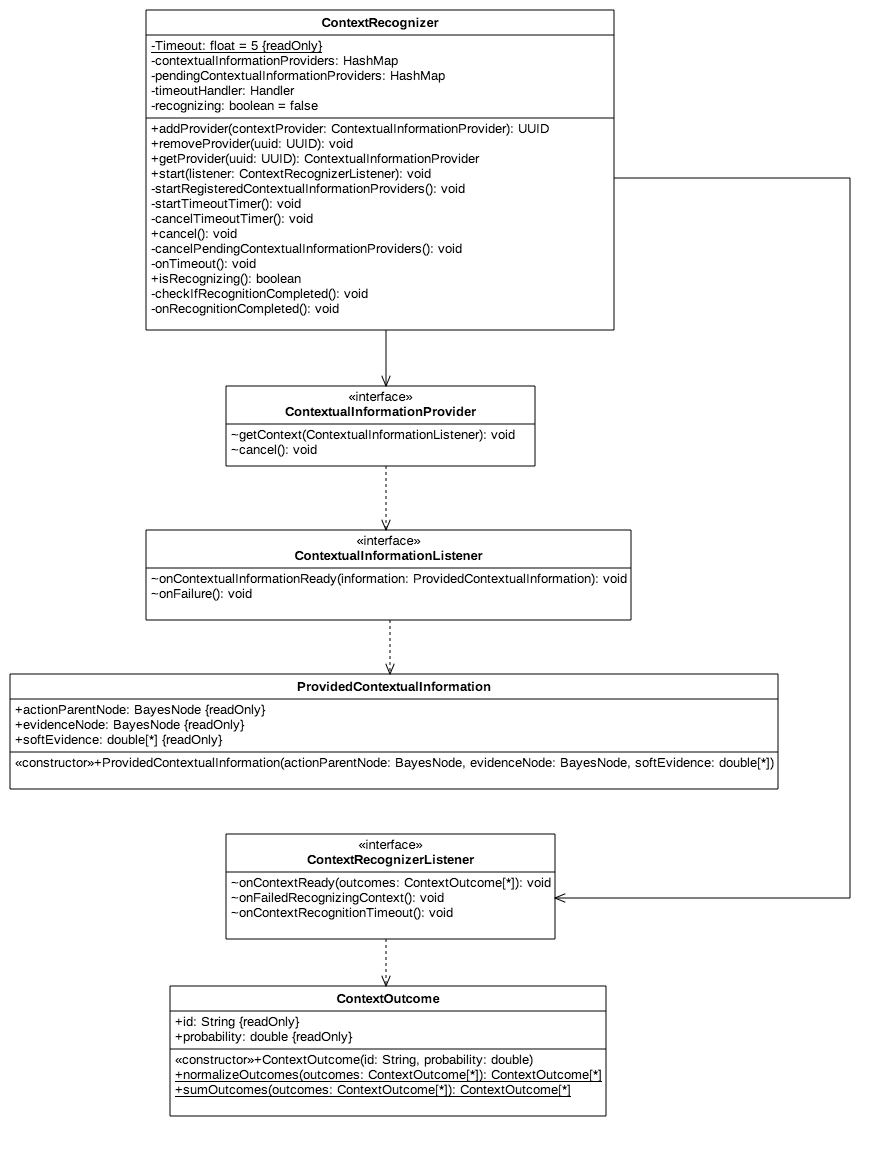
\includegraphics[width=\textwidth]{images/uml-context-engine}
\caption{Class diagram showing all classes and interfaces involved in the context engine.}
\label{fig:implementation:context-engine}
\end{figure}

\Cref{fig:implementation:context-engine:providers} shows a class diagram of the contextual information providers registered with the context recognizer in the prototype developed during the project. Below is a brief description of the classes and interfaces.

\begin{description}
\item[Beacon] A representation of a beacon installed in a room. Beacons are retrieved from openHAB over HTTP using the REST API.
\item[Room] A representation of a room which the user can be in. Rooms are retrieved from openHAB over HTTP using the REST API.
\item[PositionManager] The manager continuously listens for changes to the users position using the Estimote SDK. Based on RSSI measurements received by the Estimote SDK, the manager determines which room the user is in.
\item[EventListener] Part of the \texttt{PositionManager}. Objects conforming to the interface can be informed when the manager registers the user in a room.
\item[GestureContextualInformationProvider] Encapsulates the Gesture and Gesture\_Action nodes in the Bayesian network presented in \Cref{sec:design:bayesian-network}. When gesture recognition ends, the provider is updated with the matches which it stores and use to compute the evidence when asked to provide its contextual information as described in \Cref{sec:design:bayesian-network:gesture-node-evidence}.
\item[PositionContextualInformationProvider] Encapsulates the Room and Room\_Action nodes in the Bayesian network. Based on the observations made by the \texttt{PositionManager}, the provider calculates probabilities for the user being in each room as described in \Cref{sec:design:bayesian-network:room-node-evidence}.
\end{description}

\begin{figure}[h!]
\centering
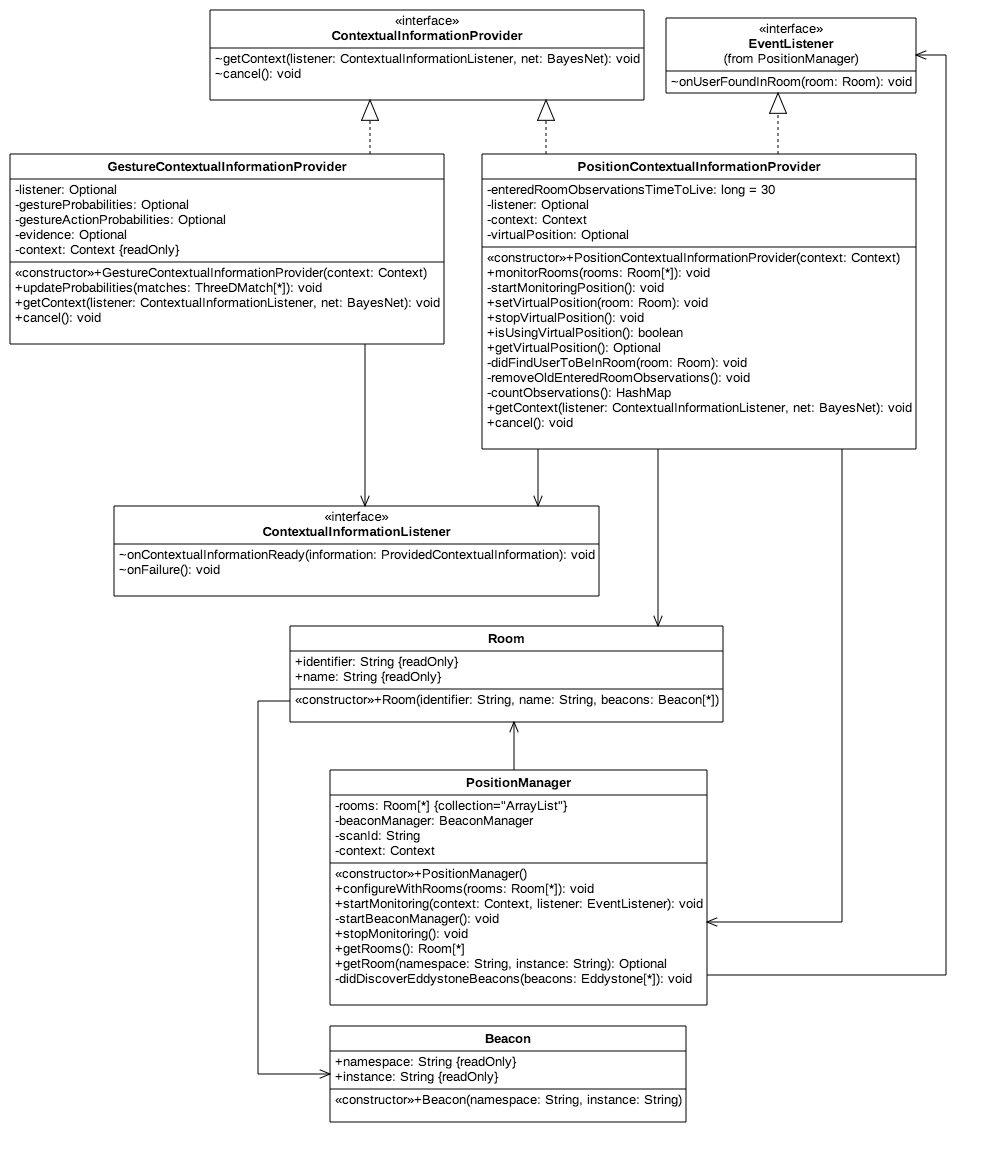
\includegraphics[width=\textwidth]{images/uml-context-engine-providers}
\caption{Class diagram showing the classes and interfaces involved in the providers.}
\label{fig:implementation:context-engine:providers}
\end{figure}

%%% Local Variables:
%%% mode: latex
%%% TeX-master: "../../master"
%%% End:

\section{Communication with openHAB}
\label{sec:design:communication-with-openhab}

The open source home automation hub openHAB described in \Cref{sec:analysis:choice-of-hub} exposes an API with a REST architecture. Clients can communicate with the API over HTTP.

The communication with the openHAB API consists of the following two components.

\begin{description}
\item[REST client] A base REST client suitable for communicating with a REST API which carries its data using JSON. The client implements base methods for interacting with a REST API. This includes retrieving, deleting, updating and creating entities. The base client parses data received by the API into models.
\item[openHAB client] The client builds on top of the base REST client and adds openHAB specific methods. This includes retrieving things and items as well as updating the state of an item.
\end{description}

\Cref{fig:design:communication-with-openhab:class-diagram-rest-client} shows a class diagram of the REST client. The involved components are briefly described below.

\begin{description}
\item[RESTClient] The base REST client which is responsible for performing requests and mapping response to models that can be further processed or displayed in the application.
\item[RequestQueue] Responsible for creating worker threads for network requests.
\item[ResultListener] Interface implemented by objects that should receive a result when a network request completes, either because of a failure or because of a succesful response.
\item[EntityBuilder] Interface implemented by objects mapping from the received JSON to models.
\item[Result] Encapsulates a network result. A result can either be a success or a failure. In case of a success, the result will contain a the value received from the API. In case of a failure, the result must contain an error.
\end{description}

\begin{figure}[h!]
\centering
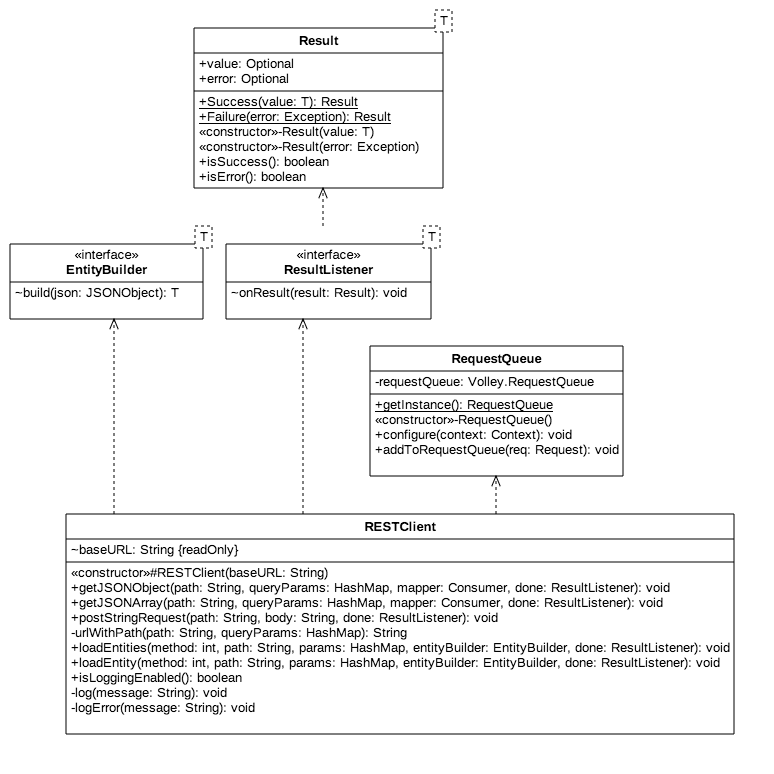
\includegraphics[width=\textwidth]{images/uml-rest-client}
\caption{Class diagram showing the architecture of the REST client used for communicating with a REST API.}
\label{fig:design:communication-with-openhab:class-diagram-rest-client}
\end{figure}

\Cref{fig:design:communication-with-openhab:class-diagram-openhab-client} shows a class diagram of the openHAB client. The involved components are briefly described below.

\begin{description}
\item[OpenHABClient] A specialization of the base REST client implementing openHAB specific functionality.
\item[BooleanResult] Similar to the Result, this either represents a success or a failure. In the case of a success, the BooleanResult does not contain a value.
\item[Item] Model representing an item in openHAB.
\item[Thing] Model representing a thing in openHAB.
\end{description}

\begin{figure}[h!]
\centering
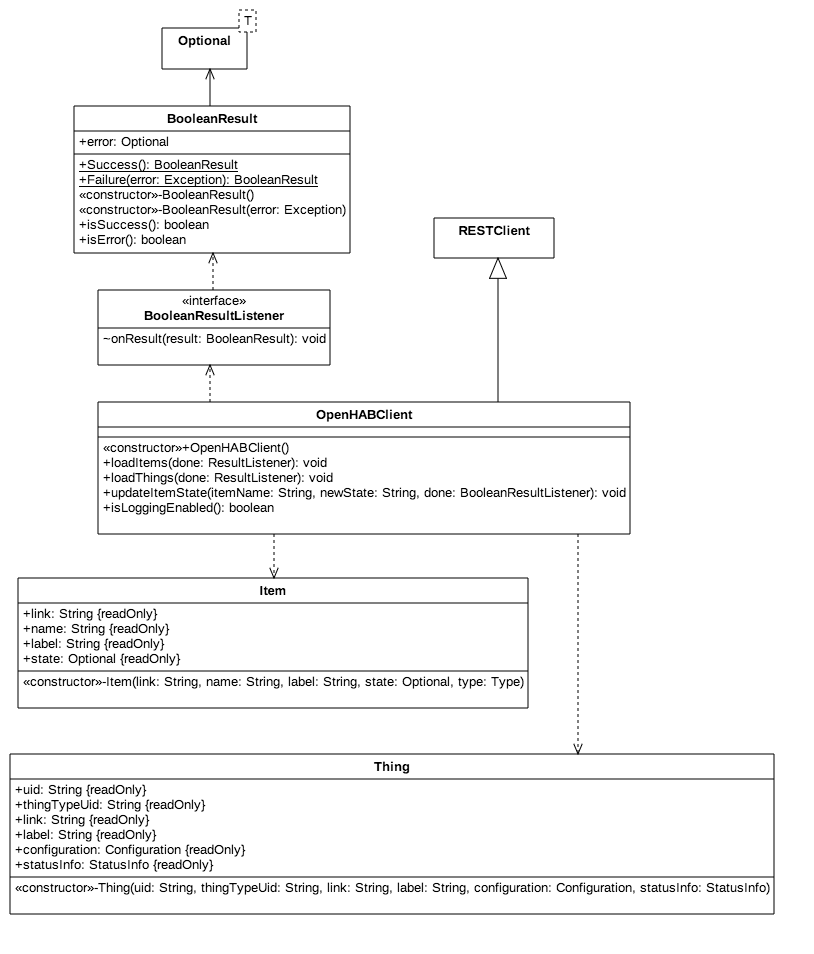
\includegraphics[width=\textwidth]{images/uml-openhab-client}
\caption{Class diagram showing the architecture of the openHAB client used for communicating with the openHAB API}
\label{fig:design:communication-with-openhab:class-diagram-openhab-client}
\end{figure}

\subsection{Mapping of Actions}

Eclipse SmartHome, which openHAB builds on top of, has a set of supported item types. An item type defines which actions an item supports. \Cref{tbl:design:communication-with-openhab:types} shows a list of the item types supported by Eclipse SmartHome and thus also by openHAB. For each item type, the actions supported by the item type is listed. Item types DateTime and Group are special items in openHAB which has no support for actions but is used to hold a date and time and a group of other items respectively.
The action types ``Percent'', ``HSB'', ``Decimal'' and ``String'' are not exact actions that can be send to openAB but refers to type of action, e.g. a lamp supporting the ``Percent'' action can receive a request containing ``50'' and adjust its brightness to 50\%. The other action types are exat actions that can be send in a request to openHAB.

In the smart watch application, we create a list of supported actions for each item. A supported action for an item is represented as the string, which is sent to openHABs API when an action should be triggered. For example, an item of type Switch has the set of actions $\{ "ON", "OFF" \}$. For the sake of this prototype, we only support a limited subset of item types and actions. The supported types and actions are shown in \Cref{tbl:design:communication-with-openhab:types}.

\begin{table}[]
\centering
\caption{Supported actions for each item type in openHAB \cite{eclipse:smarthomeitems}.}
\label{tbl:design:communication-with-openhab:types}
\begin{tabular}{p{2cm}p{6cm}p{6cm}}
\textbf{Item type} & \textbf{Description}                              & \textbf{Action types}                      \\ 
Color              & Color information (RGB)                           & ON, OFF, INCREASE, DECREASE, Percent, HSB      \\
Contact            & Item storing status of e.g. door/window contacts  & OPEN, CLOSE                                  \\
DateTime           & Stores date and time                              &                                            \\
Dimmer             & Item carrying a percentage value for dimmers      & ON, OFF, INCREASE, DECREASE, Percent           \\
Group              & Item to nest other items / collect them in groups &                                            \\
Number             & Stores values in number format                    & Decimal                                    \\
Player             & Allows to control players (e.g. audio players)    & PLAY, PAUSE, NEXT, PREVIOUS, REWIND, FASTFORWARD \\
Rollershutter      & Typically used for blinds                         & UP, DOWN, STOP, MOVE, Percent                  \\
String             & Stores texts                                      & String                                     \\
Switch             & Typically used for lights (on/off)                & ON, OFF                                     
\end{tabular}
\end{table}

\begin{table}[]
\centering
\caption{Actions supported by the smart watch application.}
\label{tbl:design:communication-with-openhab:supported-types}
\begin{tabular}{p{2cm}p{11cm}}
\textbf{Item type}      & \textbf{Action types}                      \\ 
Dimmer                  & ON, OFF, INCREASE, DECREASE, 10, 20, 30, 40, 50, 60, 70, 80, 90           \\
Switch                  & ON, OFF                                     
\end{tabular}
\end{table}

%%% Local Variables:
%%% mode: latex
%%% TeX-master: "../../master"
%%% End:

\section{Prototype}
\label{sec:implementation:prototype}

This section presents the prototype of the Android Wear application as well as the \emph{binding}, i.e. an addon providing functionality specific to a problem domain, for openHAB developed during the project.

\subsection{Android Wear}
\label{sec:implementation:prototype:android-wear}

\Cref{fig:implementation:prototype:navigation-diagram} shows a navigation diagram of the smart watch application. The letters in the top right corner of the nodes in the diagram references the screenshots shown in \Cref{fig:implementation:prototype:screenshots}.

The diagram shows that the application can be considered divided into the following two areas.

\begin{description}
\item[Primary use] We refer to the parts of the application which the user use the most as the \emph{primary use}. This involves the recognition of gestures as well as the picker presented when an action to trigger could not be determined after context recognition.
\item[Configuration] Before the user gets involved with the primary use, he will need to configure the application, i.e. train gestures and create gesture configurations.
\end{description}

When opening the application, the user is presented with a screen to perform gesture recognition. This enables the user to start context recognition fast, whereas he needs to dive deeper into the navigation in order to train gestures and create gesture configurations, i.e. features that he will not use as often as the context recognition.

For a list of the supported features in the application, please refer to \Cref{sec:implementation:status}.

\begin{figure}[!htb]
    \centering
    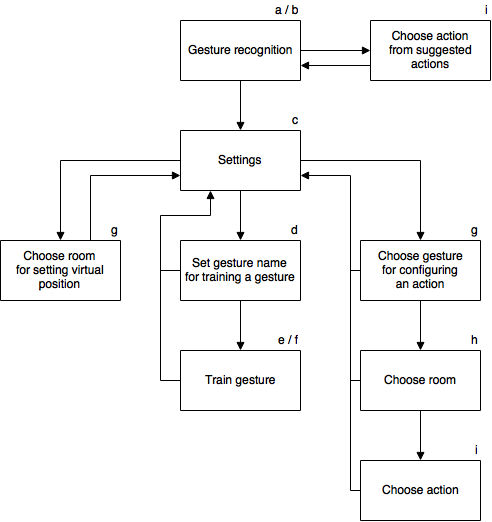
\includegraphics[width=0.7\textwidth]{images/wear-navigation-diagram}
    \caption{Navigation diagram of the application developed for the Android Wear device. Letters in the top right corner of each node refers to the screenshots in figure \Cref{fig:implementation:prototype:screenshots}.}
    \label{fig:implementation:prototype:navigation-diagram}
\end{figure}

\begin{figure}[!htb]%
    \centering
    \subbottom[Screen on which the user can start gesture recognition by touching the screen.]{\label{fig:implementation:protoype:screenshots:1}
        \frame{
\includegraphics[width=0.3\textwidth]{images/wear-screenshot-touch-recognize}}
    }
    \subbottom[Screen on which the user can stop gesture recognition by touching the screen. The orange color indicates that recognition has been started.]{\label{fig:implementation:prototype:screenshots:2}
        \frame{
\includegraphics[width=0.3\textwidth]{images/wear-screenshot-recognizing}}
    }
    \subbottom[Settings screen from which the user can set his virtual, train a gesture and configure a new action (create a gesture configuration). When a virtual position is set, the setting can be selected again to unet the virtual position.]{\label{fig:implementation:prototype:screenshots:3}
        \frame{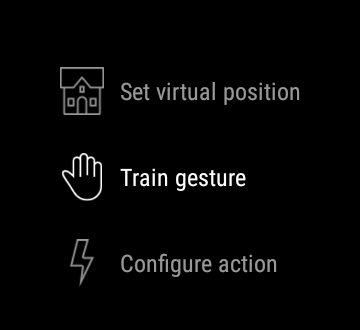
\includegraphics[width=0.3\textwidth]{images/wear-screenshot-settings}}
    }
    \subbottom[Screen shown when the user starts training a gesture. Tapping the ``Gesture name'' button will present the user with a speech recognition interface from which he pronounce the name of the gesture to configure it.]{\label{fig:implementation:protoype:screenshots:4}
        \frame{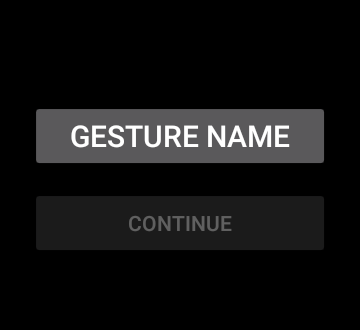
\includegraphics[width=0.3\textwidth]{images/wear-screenshot-name-gesture}}
    }
    \subbottom[Screen shown when training a gesture and the gesture recognizer has not been started. We see that two gesture samples, i.e. gesture templates, have been trained.]{\label{fig:implementation:prototype:screenshots:5}
        \frame{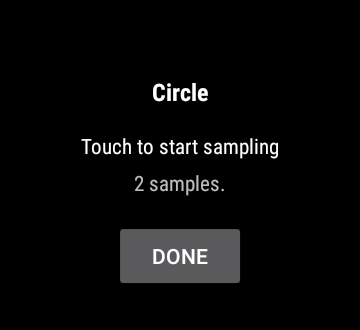
\includegraphics[width=0.3\textwidth]{images/wear-screenshot-touch-train}}
    }
    \subbottom[Screen shown when training a gesture and the gesture recognizer has been started, i.e. the user is performing a gesture.]{\label{fig:implementation:prototype:screenshots:6}
        \frame{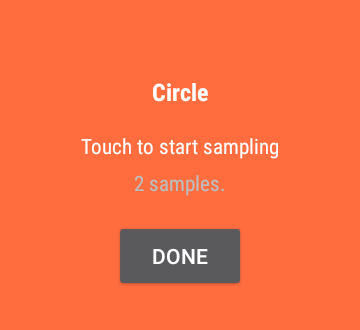
\includegraphics[width=0.3\textwidth]{images/wear-screenshot-training}}
    }
    \subbottom[Gesture picker showing the gestures the user has trained. The gesture picker is used when creating a gesture configuration.]{\label{fig:implementation:protoype:screenshots:7}
        \frame{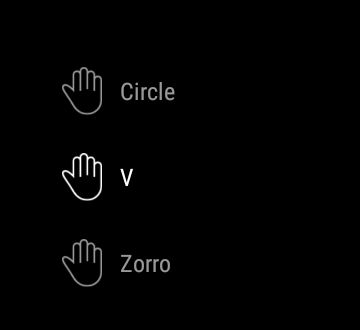
\includegraphics[width=0.3\textwidth]{images/wear-screenshot-gestures}}
    }
    \subbottom[Room picker shown when the user creates a gesture configuration. The picker is also shown when setting a virtual position.]{\label{fig:implementation:prototype:screenshots:8}
        \frame{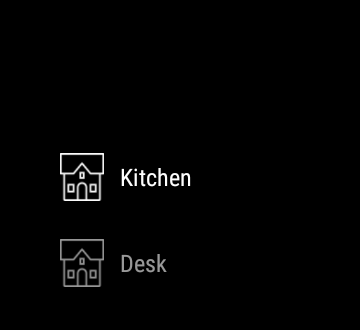
\includegraphics[width=0.3\textwidth]{images/wear-screenshot-rooms}}
    }
    \subbottom[Action picker shown when creating a gesture configuration. A similar picker is shown when the context engine suggests multiple actions.]{\label{fig:implementation:prototype:screenshots:9}
        \frame{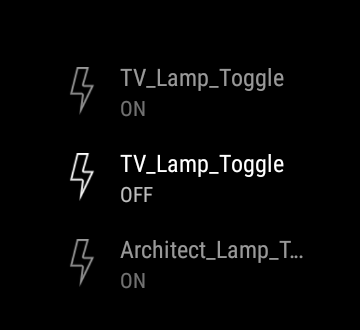
\includegraphics[width=0.3\textwidth]{images/wear-screenshot-actions}}
    }
    \caption{Screenshots of the prototype developed for the Android Wear smart watch.}
    \label{fig:implementation:prototype:screenshots}
\end{figure}

\subsection{openHAB}
\label{sec:implementation:prototype:openhab}

We developed a \emph{binding} for openHAB. A \emph{binding} is an addon for openHAB which relates to a specific problem domain. For example, there is a binding for communcating with Philips Hue lights and a binding for controlling a Sonos media centre. We have created a binding for configuring the rooms and beacons in a users home.

We chose to place the configuration of the rooms and beacons in openHAB, as this is a one time configuration which can be shared amongst the users in a home where as the creation of gesture configurations is place on the watch as this can be independent for each inhabitant of a home.

The rooms and beacons are synchronized to the smart watch when the application is loaded. The watch use the models when positioning the user.

A room has a name and when it is created, openHAB assigns it a UID. When creating a beacon, the user must enter the UID assigned by openHAB in order to specify which room the beacon is placed in. Furthermore the user should enter the Eddystone namespace and instance, both described in \Cref{sec:design:ble-positioning}. This identifies the specific beacon. When the smart watch registers a beacon, it can determine which room the user is in by the beacons reference to a room.

% \begin{figure}[!htb]%
%     \centering
%     \subbottom[Screen on which to choose the binding to configure.]{\label{fig:implementation:protoype:openhab:bindings}
%         \frame{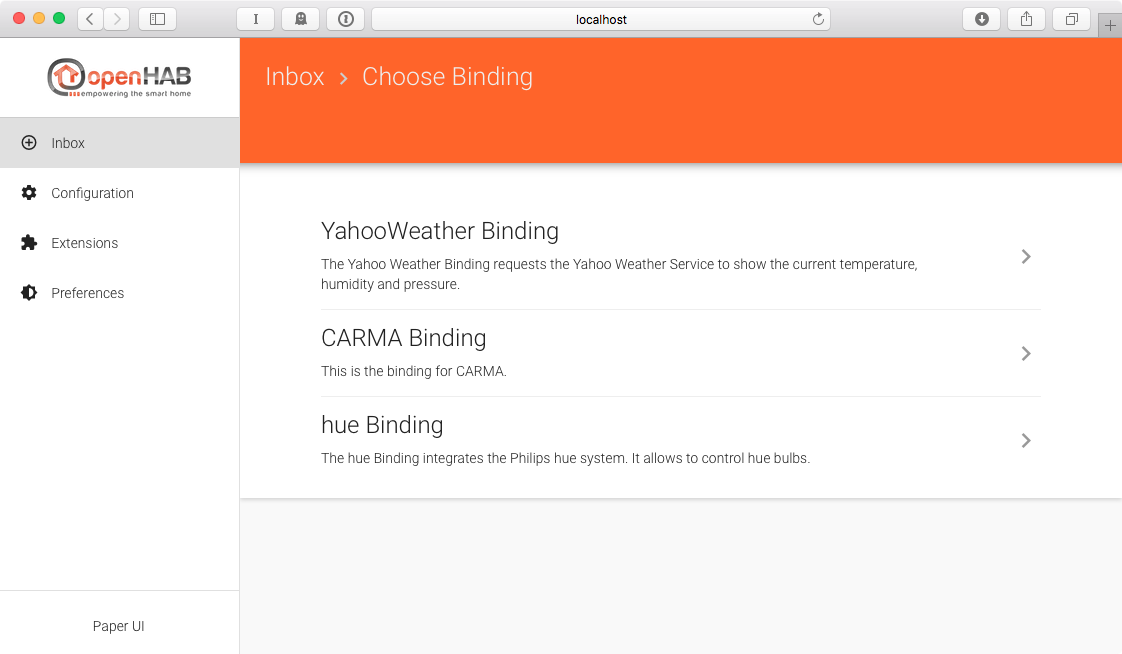
\includegraphics[width=0.5\textwidth]{images/openhab-addon-bindings}}
%     }
%     \subbottom[Screen on which the \emph{thing} to create is chosen. In openHAB physical devices are referred to as \emph{things}.]{\label{fig:implementation:prototype:openhab:things}
%         \frame{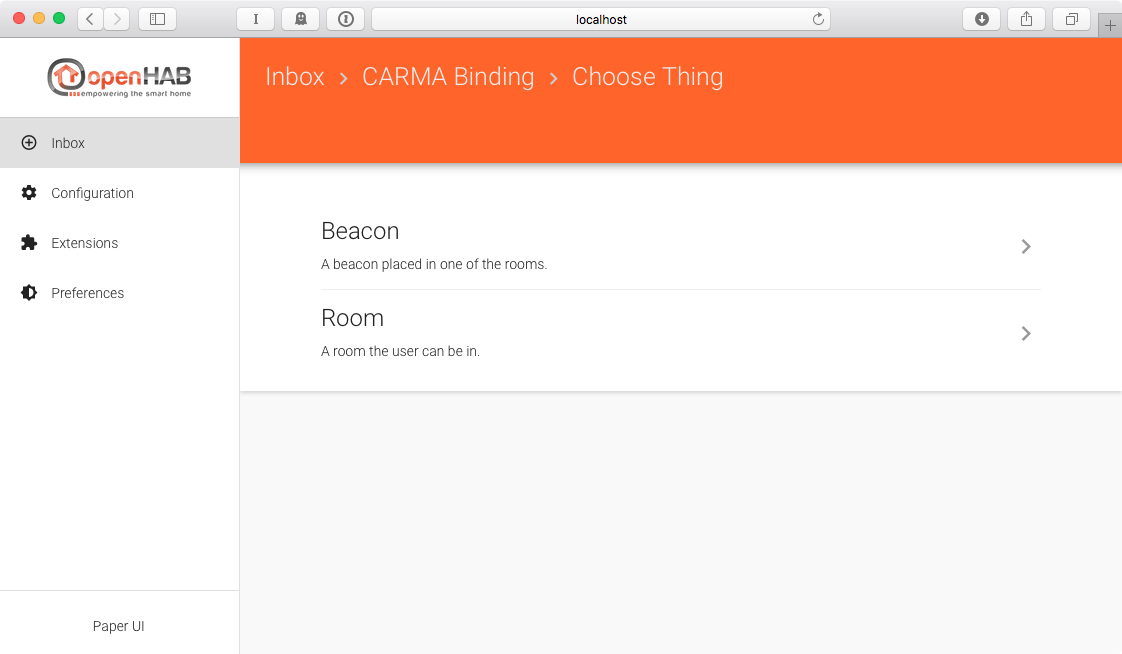
\includegraphics[width=0.45\textwidth]{images/openhab-addon-things}}
%     }
%     \subbottom[Screen on which a new room can be created. The room should have a name, e.g. ``Kitchen'' or ``Living room''.]{\label{fig:implementation:protoype:openhab:room}
%         \frame{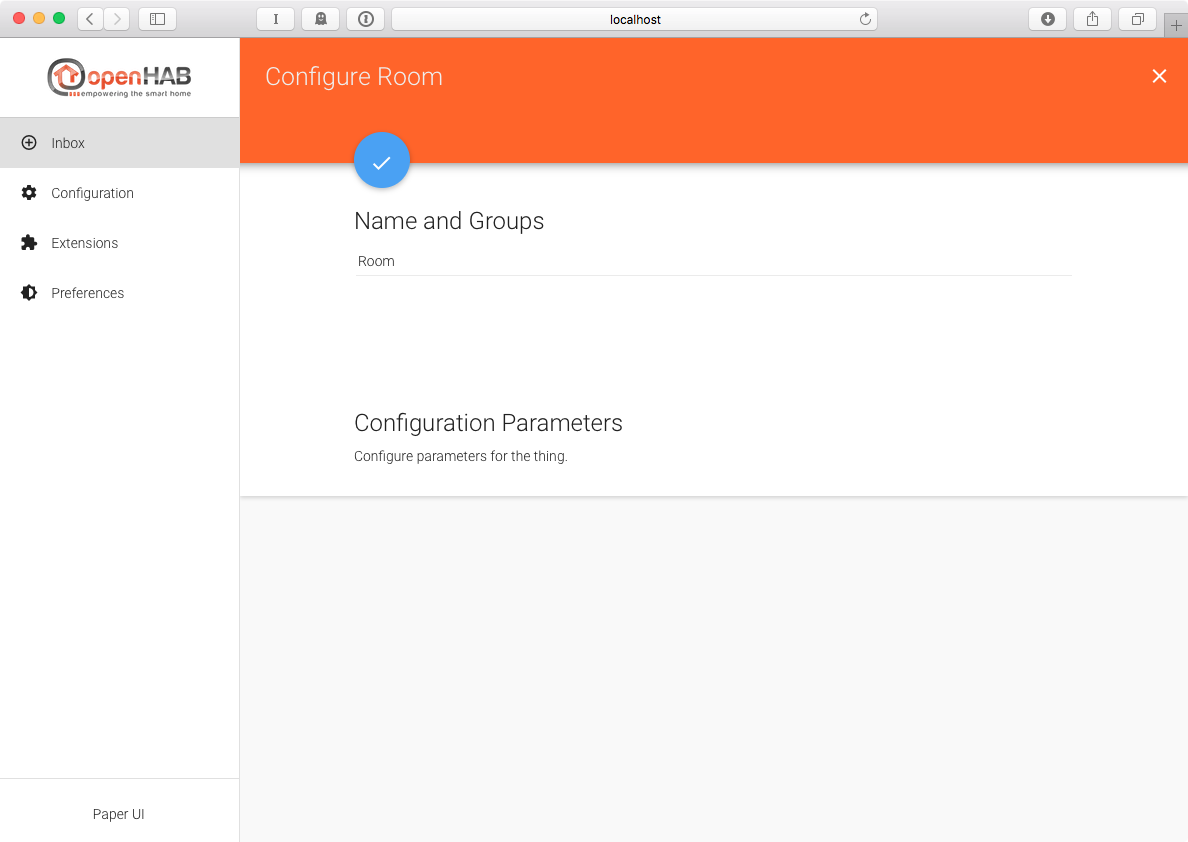
\includegraphics[width=0.45\textwidth]{images/openhab-addon-room}}
%     }
%     \subbottom[Screen on which a new beacon can be created. The UID of the room the beacon is placed in must be specified. UIDs are created by openHAB when a new room is created. The namespace and instance of the Eddystone beacon must also be specified. ]{\label{fig:implementation:prototype:openhab:beacon}
%         \frame{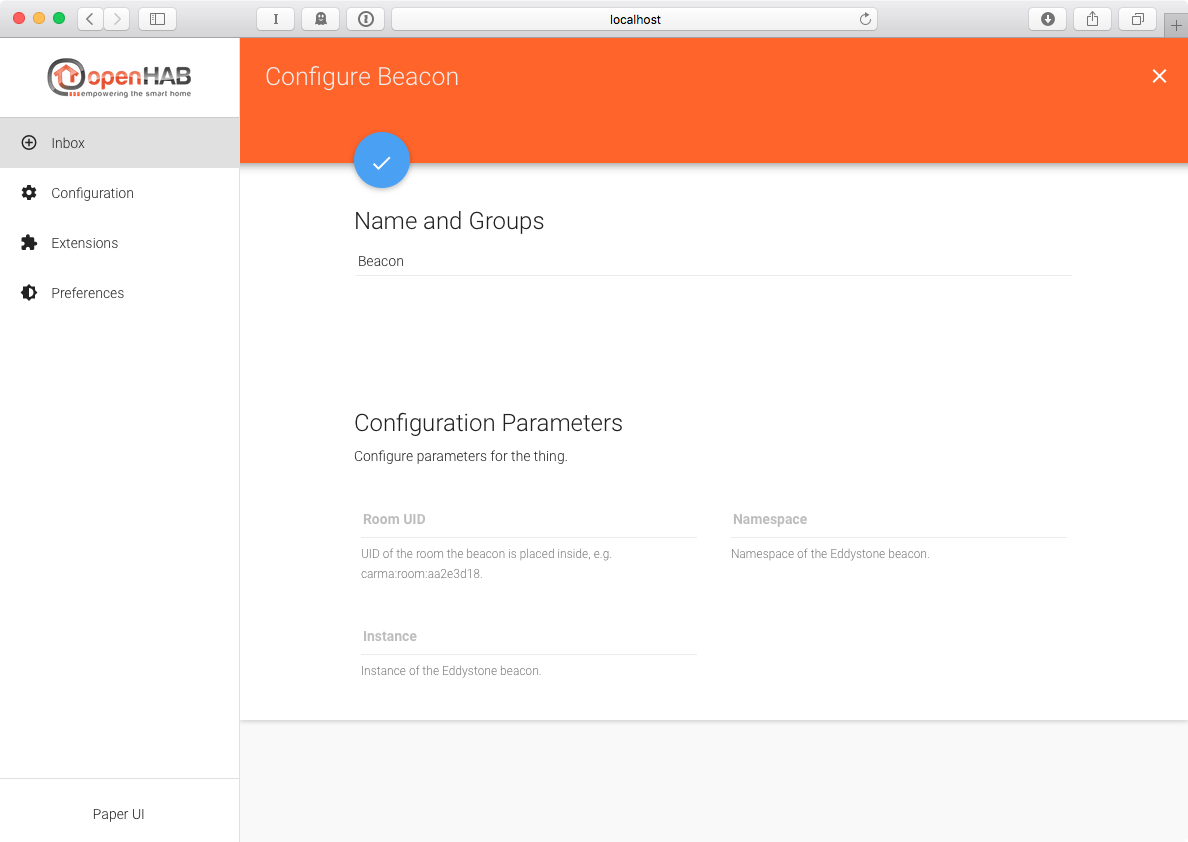
\includegraphics[width=0.45\textwidth]{images/openhab-addon-beacon}}
%     }
%     \subbottom[Screen showing the list of all configured things in openHAB. The screenshot shows two rooms and two beacons configured as well as some Philips Hue light bulbs.]{\label{fig:implementation:prototype:openhab:list}
%         \frame{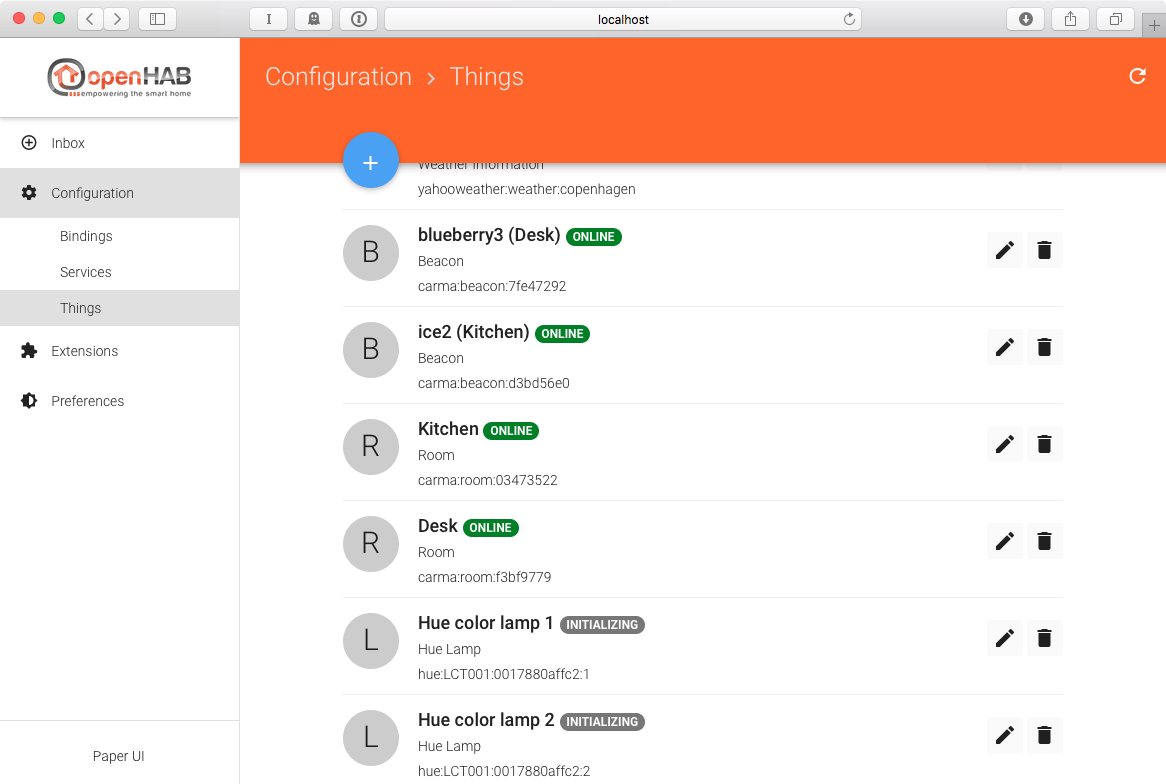
\includegraphics[width=0.45\textwidth]{images/openhab-addon-list}}
%     }
%     \caption{Screenshots of the binding developed for openHAB.}
%     \label{fig:implementation:prototype:openhab:screenshots}
% \end{figure}

%%% Local Variables:
%%% mode: latex
%%% TeX-master: "../../master"
%%% End:


%%% Local Variables:
%%% mode: latex
%%% TeX-master: "../master"
%%% End:
